\documentclass[10pt]{article}

\usepackage[verbose,tmargin=1in,bmargin=1in,lmargin=1in,rmargin=1in]{geometry}
% \usepackage[margin=0.5in,bottom=.7in,top=.8in]{geometry}
\usepackage{graphicx}\graphicspath{{figures/}}
\usepackage{amsmath}
\usepackage[usenames,dvipsnames]{color}
\usepackage[colorlinks=true,citecolor=Mahogany,linkcolor=Mahogany,urlcolor=Mahogany,filecolor=Mahogany]{hyperref}
\usepackage{breakurl}
\usepackage{url}
\usepackage[nocompress]{cite}
\usepackage{verbatim}
\usepackage{paralist}
\usepackage{authblk}
\usepackage{listings}

\graphicspath{{figures/}}

\title{(PRELIMINARY DRAFT) NDN Technical Memo: LINK}

\author{NDN Project Team}

% \date{NDN Project Team}
\date{}

% \usepackage{eso-pic,xcolor}
% \makeatletter
% \AddToShipoutPicture*{%
% \setlength{\@tempdimb}{20pt}%
% \setlength{\@tempdimc}{\paperheight}%
% \setlength{\unitlength}{1pt}%
% \put(\strip@pt\@tempdimb,\strip@pt\@tempdimc){%
%     \makebox(0,-60)[l]{\color{blue}%
% NDN, Technical Report NDN-0022. \url{http://named-data.net/techreports.html}}
%   }%
% }
% \makeatother


\begin{document}
\maketitle

% \section*{Revision history}

% \begin{center}
% \begin{tabular}{|l|l|p{10cm}|}
% \hline
% \bf Revision & \bf Revision date & \bf Description \\
% \hline
% 1 & July 21, 2014 & Initial release \\
% \hline
% \end{tabular}
% \end{center}

\section{Introduction}

This document defines LINK object and its usage.

\section{LINK Object}

\subsection{LINK for Redirect}

By its name, a LINK object binds together two names (a name can be a prefix).
In a way, this is somewhat similar to the ``symbolic link'' in UNIX file system.

We define LINK as a sub-type of NDN DATA packet (Figure~\ref{fig:link}). In this DATA packet,

\begin{figure}[h]
  \centering
  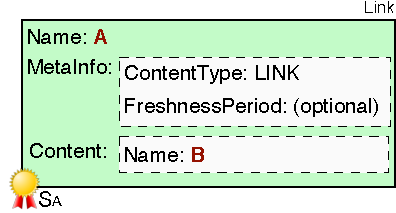
\includegraphics[scale=0.8]{ndn-link}
  \caption{Link}
  \label{fig:link}
\end{figure}


\begin{itemize}
\item \textbf{Name:} $\mathtt{Name}_A$
\item \textbf{MetaInfo:}
  \begin{itemize}
  \item \textbf{ContentType:} \verb|LINK|
  \item \textbf{FreshnessPeriod:} optional, producer defined period of LINK object freshness
  \end{itemize}
\item \textbf{Content:} $\mathtt{Name}_B$
\item \textbf{Signature:} by a key that authorized to sign Data in namespace $\mathtt{Name}_A$.
  For example, in the hierarchical trust model, this is $\mathtt{Name}_A$ or $\mathtt{Name}_A$ 's parent key, confirming that $\mathtt{Name}_A$ has delegated a sub-namespace to $\mathtt{Name}_B$
\end{itemize}

This LINK object binds together the names A and B.

LINK can be used to serve two purposes: redirect (like HTTP redirect), or encapsulation.

``Redirect'' means that when a consumer sends an Interest with name $\mathtt{Name}_A$, the reply Data packet contains a LINK which carries another name $\mathtt{Name}_B$, indicating that the produce of $\mathtt{Name}_A$ suggests the consumer to send the Interest using name B to request the desired data.
Here $\mathtt{Name}_A$ and $\mathtt{Name}_B$ can be either a prefix or an exact name

\subsection{LINK with Delegation}

In many cases, it is necessary to ensure not only that an entity A has linked some name prefix from namespace A to namespace B, but also that B has authorized A to perform such actions.
For this purpose we define Delegation link object (Figure~\ref{fig:delegation}), which contains the following information:

\begin{figure}[h]
  \centering
  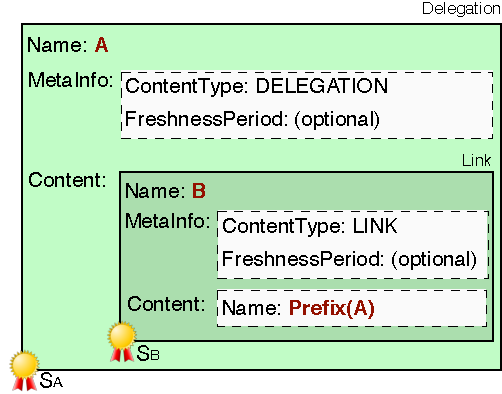
\includegraphics[scale=0.8]{delegation}
  \caption{Delegation}
  \label{fig:delegation}
\end{figure}

\begin{itemize}
\item \textbf{Name:} $\mathtt{Name}_A$
\item \textbf{MetaInfo:}
  \begin{itemize}
  \item \textbf{ContentType:} \verb|DELEGATION|
  \item \textbf{FreshnessPeriod:} optional, producer defined period of DELEGATION object freshness
  \end{itemize}
\item \textbf{Content:} LINK object ``redirecting'' namespace $B$ to a prefix of name $A$.  This LINK object ensures that owner of namespace $B$ actually authorized owner of the namespace $A$ to perform redirections.
\item \textbf{Signature:} by a key that authorized to sign Data in namespace $\mathtt{Name}_A$.
  For example, in the hierarchical trust model, this is $\mathtt{Name}_A$ or $\mathtt{Name}_A$ 's parent key, confirming that $\mathtt{Name}_A$ has delegated a sub-namespace to $\mathtt{Name}_B$
\end{itemize}



\subsection{LINK for Data Retrieval (Encapsulation)}

``Encapsulation'' is needed when consumer wants to fetch Data whose prefix $P_u$ is not announced to the routing system.
To be able to fetch this Data, there must be a routable prefix $P_r$ so that a certain way of concatenating $P_r|P_u$ can get the desired data back.

More specifically, to retrieve a Data packet with a name $N_{u}$ that is not directly routable towards producer, a consumer needs to perform the following steps:

\begin{itemize}
\item perform a resolution $N_i \Rightarrow P_r$ (e.g., using NDNS), which should return a LINK object defined in the previous section.
  This LINK is binding an unroutable prefix of $N_i$ (this prefix can/will be discovered during resolution process) to routable prefix $P_r$.
\item construct the name $N_{r}$ that contains $P_r$ and $N_{u}$ (e.g., concatenation or concatenation with marker delimiter\footnote{The delimiter may be necessary to disambiguate prefixes during forwarding}), and sends Interest packet
\end{itemize}

The retrieved Data packet should conform to the following format (Figure~\ref{fig:linked-data}):

\begin{figure}[h]
  \centering
  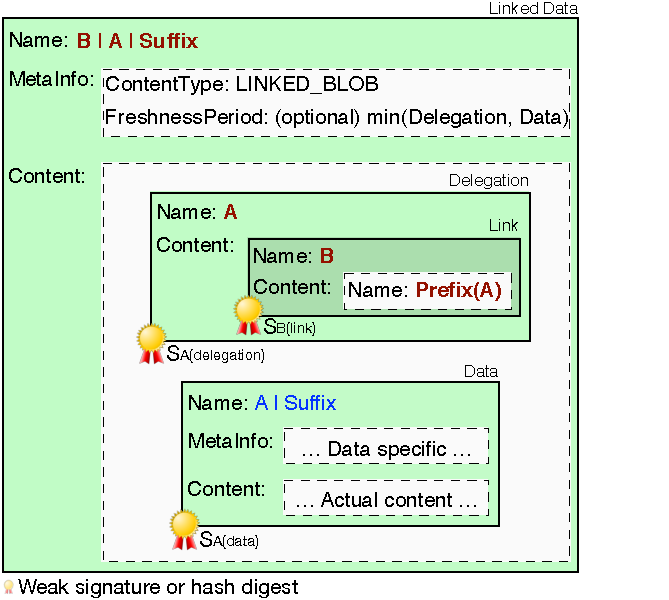
\includegraphics[scale=0.8]{linked-data}
  \caption{Linked Data}
  \label{fig:linked-dat}
\end{figure}

\begin{figure}[h]
  \centering
  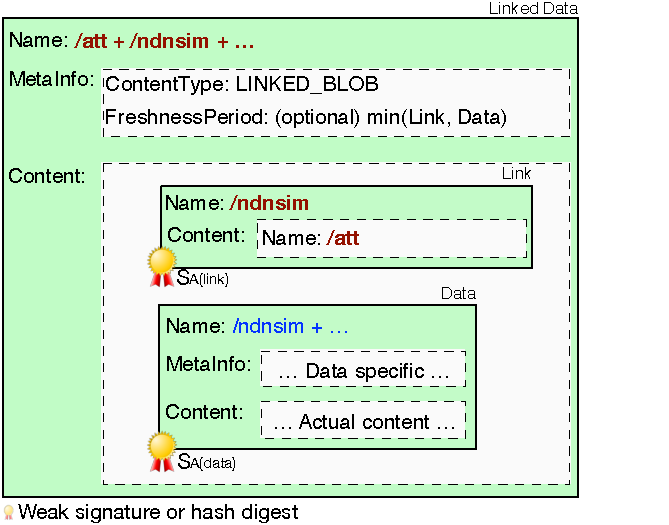
\includegraphics[scale=0.8]{linked-data2}
  \caption{Linked Data 2}
  \label{fig:linked-dat}
\end{figure}

\begin{itemize}
\item \textbf{Name:} $\mathtt{Name}_{outer}$
\item \textbf{MetaInfo:}
  \begin{itemize}
  \item \textbf{ContentType:} \verb|LINKED_BLOB|
  \item \textbf{FreshnessPeriod:} optional, $\min(\mathtt{FreshnessPeriod}_{LINK}, \mathtt{FreshnessPeriod}_{BLOB})$
  \end{itemize}
\item \textbf{Content:} two Data packets stacked together
  \begin{itemize}
  \item Delegation object linking Pr to Pu
  \item Data object with name N1 that the consumer wants, and with a signature by N1 or its parent's key.
  \end{itemize}

\item \textbf{Signature:} lightweight signature by $\mathtt{Name}_{outer}$ owner or hash digest for transmission integrity protection.

\end{itemize}


\subsubsection{Details to Work Out}


Details on how $\mathtt{Name}_{outer}$ is constructed is TBD.

% \bibliographystyle{plain}
% \bibliography{link}

\end{document}
